  \documentclass[11pt,a4paper]{article}
  \usepackage[utf8]{inputenc}
  \usepackage[T1]{fontenc}
  \usepackage{geometry}
  \usepackage{graphicx}
  \usepackage{hyperref}
  \usepackage{booktabs}
  \usepackage{parskip}
  \usepackage{tikz}
  \usetikzlibrary{shapes.geometric, arrows.meta, positioning}
  \geometry{margin=2.5cm}

  \title{Web Mining and Semantics\\Lab Report: From Unstructured Web to Knowledge Base}
  \author{Student Project}
  \date{\today}

  \begin{document}
  \maketitle

  %=============================================================================
  \section{Introduction}
  %=============================================================================

  This report describes a two-phase pipeline for building a Knowledge Base (KB) in the domain of \textbf{Local History}, from raw web data to a structured RDF graph aligned with Linked Open Data (LOD). The objective is to transform unstructured text into triples suitable for Knowledge Graph Embedding (KGE).

  \textbf{Domain and sources.} We focus on cultural heritage objects (monuments, historical figures, places) using the \textbf{Europeana API} as the primary data source. Europeana provides metadata for millions of digitized cultural items; we extract text from the Search API JSON response rather than scraping HTML, which avoids anti-robot issues and simplifies content extraction.

  \textbf{Scope.} Phase~1 covers crawling, cleaning, Named Entity Recognition (NER), and Relation Extraction (RE). Phase~2 covers KB construction, entity and predicate alignment with Wikidata/DBpedia, and expansion via SPARQL to reach the target volume (50k--200k triplets, 5k--30k entities, 50--200 relations). Phase~3 adds knowledge reasoning: SWRL rule-based inference with OWLReady2 and Pellet, and Knowledge Graph Embedding (KGE) with TransE and ComplEx for link prediction.

  %=============================================================================
  \section{Phase 1: From Unstructured Web to Structured Entities}
  %=============================================================================

  \subsection{Methodology and Pipeline}

  The extraction pipeline follows four main stages: (1) source selection and crawling, (2) content extraction and cleaning, (3) named entity recognition, and (4) relation extraction.

  \textbf{Source selection.} As recommended in the instructions, we use APIs when anti-robot checking occurs. The primary source is the \textbf{Europeana API} (Search API at \texttt{api.europeana.eu}), which provides metadata and descriptions for cultural heritage objects (Local History domain). No scraping or trafilatura is needed for API-sourced content; text is extracted directly from the JSON response and enriched with additional textual metadata fields.

  \textbf{Content extraction.} Text comes from Europeana API responses and is normalized (whitespace cleanup, URL literal filtering). A strict useful-page threshold is applied: items with fewer than 500 words are discarded, in line with the challenge requirement of Phase~1.

  \textbf{Storage.} Results are stored in JSONL format, with one JSON object per line containing \texttt{url}, \texttt{text}, \texttt{title}, and \texttt{word\_count}.

  \textbf{NER.} We use spaCy with the \texttt{en\_core\_web\_trf} model (transformer-based) to extract entities of type PERSON, ORG, GPE, and DATE. Common nouns and generic terms are filtered out.

  \textbf{Relations.} For each sentence containing at least two entities, we use dependency tags (\texttt{nsubj}, \texttt{dobj}, \texttt{pobj}) to find a verb connecting them. The verb lemma is used as the predicate for triples of the form (subject, predicate, object).

  \begin{figure}[ht]
  \centering
  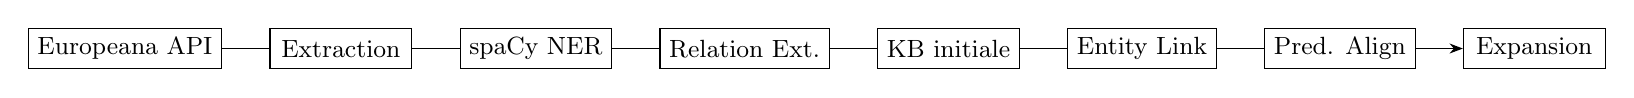
\begin{tikzpicture}[
    node distance=0.6cm,
    box/.style={rectangle, draw, minimum width=1.8cm, minimum height=0.5cm, font=\small},
    arrow/.style={-Stealth}
  ]
    \node[box] (api) {Europeana API};
    \node[box, right=of api] (extract) {Extraction};
    \node[box, right=of extract] (ner) {spaCy NER};
    \node[box, right=of ner] (re) {Relation Ext.};
    \node[box, right=of re] (kb) {KB initiale};
    \node[box, right=of kb] (el) {Entity Link};
    \node[box, right=of el] (pa) {Pred. Align};
    \node[box, right=of pa] (exp) {Expansion};
    \draw[arrow] (api) -- (extract) -- (ner) -- (re) -- (kb) -- (el) -- (pa) -- (exp);
  \end{tikzpicture}
  \caption{Pipeline global du projet : Phase~1 (Crawling $\rightarrow$ NER $\rightarrow$ RE) et Phase~2 (KB $\rightarrow$ alignement $\rightarrow$ expansion).}
  \end{figure}

  \subsection{Choix méthodologique NER}

  We use spaCy's \texttt{en\_core\_web\_trf} model, a transformer-based approach. Compared to rule-based methods or CRF (Conditional Random Fields), transformer-based NER offers several advantages (information\_retrieval.pdf): (1) no manual feature engineering---the model learns representations from raw text; (2) context-aware encoding (e.g., ``Paris'' in ``Paris Hilton'' vs.\ ``Paris, France''); (3) end-to-end learning for entity labels. The lemmatizer integrated in spaCy normalizes verb forms (e.g., ``built'' $\rightarrow$ ``build'') for consistent predicate naming in triples.

  \subsection{Relation Extraction}

  Relation extraction follows the dependency-based approach (information\_retrieval.pdf): for each sentence with at least two entities, we use dependency tags \texttt{nsubj} (subject), \texttt{dobj} (direct object), and \texttt{pobj} (prepositional object) to find a verb connecting them. Example: ``Marie Curie discovered Polonium'' yields the triple \texttt{(Marie Curie, discovered, Polonium)}. When no verb is found but exactly two entities co-occur, we use \texttt{relatedTo} as fallback; we avoid co-occurrence-only pairs in longer lists to reduce noise.

  \begin{figure}[ht]
  \centering
  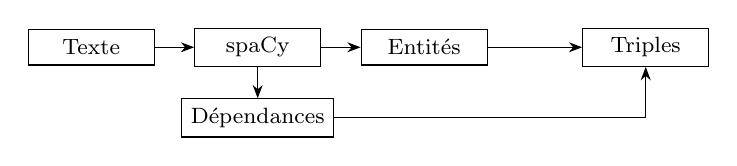
\begin{tikzpicture}[
    node distance=0.5cm,
    box/.style={rectangle, draw, minimum width=1.6cm, minimum height=0.45cm, font=\footnotesize},
    arrow/.style={-Stealth}
  ]
    \node[box] (text) {Texte};
    \node[box, right=of text] (spacy) {spaCy};
    \node[box, right=of spacy] (ents) {Entités};
    \node[box, below=0.4cm of spacy] (deps) {Dépendances};
    \node[box, right=1.2cm of ents] (triples) {Triples};
    \draw[arrow] (text) -- (spacy);
    \draw[arrow] (spacy) -- (ents);
    \draw[arrow] (spacy) -- (deps);
    \draw[arrow] (ents) -- (triples);
    \draw[arrow] (deps) -| (triples);
  \end{tikzpicture}
  \caption{Architecture NER/RE : le texte est traité par spaCy (transformer + lemmatizer) pour produire entités (PERSON, ORG, GPE, DATE) et dépendances (nsubj, dobj, pobj), puis les triples (s, p, o).}
  \end{figure}

  \subsection{Entity Ambiguity Analysis}

  Three examples of entity ambiguity:

  \begin{enumerate}
  \item \textbf{``Paris''} -- The NER can correctly identify Paris as the city (GPE) in most contexts. However, in ``Paris Hilton'' or ``Treaty of Paris,'' the same string refers to a person or a document. Context is crucial; the model may mislabel in ambiguous sentences.

  \item \textbf{``May''} -- May can be a month (DATE), a person's name (PERSON), or a modal verb. In ``The treaty was signed in May 1919,'' it is correctly a DATE. In ``May I help you?,'' it is not an entity; misclassification can occur if the model is not context-aware.

  \item \textbf{``Louis''} -- In ``Louis XIV built the Palace of Versailles,'' Louis refers to the king. In ``Louis, Missouri,'' it refers to a place. The model may also confuse ``Louis'' with ``Saint Louis'' (a person or a city). Without disambiguation, entity linking can fail.
  \end{enumerate}

  As noted in QueryWithOpenKB, ambiguity in entity lookup is common: ``Paris'' can denote Paris (France), Paris (Texas), Paris (mythology), or Paris (person). Entity alignment requires context; we use type-based filtering (GPE $\rightarrow$ place, PERSON $\rightarrow$ human) and Property Evidence when available to improve disambiguation.

  \subsection{Scaling Reflection}

  For 10,000 pages instead of 10, the approach would need several changes:

  \begin{itemize}
  \item \textbf{Parallel crawling:} Use a thread pool or \texttt{asyncio} with rate limiting to avoid overloading servers. Respect \texttt{Crawl-delay} in robots.txt when specified.

  \item \textbf{Incremental storage:} Append to JSONL instead of loading all data into memory. Use batch processing for NER and relation extraction.

  \item \textbf{Database:} Replace CSV with a database (e.g., SQLite) for large-scale entity and triple storage.

  \item \textbf{Resumability:} Track crawled URLs and skip already-processed pages. Store checkpoints for long-running jobs.

  \item \textbf{Monitoring:} Log failures and retry with exponential backoff. Monitor for blocked IPs or rate limits.
  \end{itemize}

  %=============================================================================
  \section{Phase 2: Knowledge Base Construction, Alignment, and Expansion}
  %=============================================================================

  \subsection{Alignment Strategy}

  \textbf{Entity linking.} Per instructions (DBpedia or Wikidata), we search the Wikidata API (\texttt{wbsearchentities}). When a match is found, we add \texttt{owl:sameAs} to the Wikidata entity URI (e.g.\ \texttt{wd:Q90} for Paris) with confidence from the API. Only Wikidata/DBpedia URIs are added to the alignment file---Europeana item URIs are not used for alignment, as they are not SPARQL-queryable on LOD. When Wikidata has no match, we create a new entity in the ontology with a precise type (Person, Organization, Place, Temporal) and mark it as NEW in the mapping table.

  \textbf{Disambiguation strategies (QueryWithOpenKB).} We apply: (1) \textit{Type-based filtering}: GPE $\rightarrow$ place/city, PERSON $\rightarrow$ human, ORG $\rightarrow$ organization; (2) \textit{Property Evidence}: when the API returns a description, we boost confidence if it matches the expected type; (3) \textit{Label match}: exact match yields higher confidence than partial match. DBpedia Spotlight could be used as an alternative for entity linking when text context is available.

  \textbf{Predicate alignment.} Per instructions, we use SPARQL queries on the Wikidata endpoint (\texttt{query.wikidata.org}) to find equivalent properties. For each private predicate, we run a query filtering by label (e.g.\ ``location'' for \texttt{locatedIn}) and select the most pertinent result. We use \texttt{owl:equivalentProperty} when semantics match exactly, and \texttt{rdfs:subPropertyOf} when our predicate is narrower (e.g., \texttt{wonAward} $\sqsubseteq$ \texttt{wdt:P166}). When SPARQL returns no match, we fall back to EDM/Dublin Core (e.g.\ \texttt{dcterms:spatial}, \texttt{dc:creator}).

  \subsection{Linking vs.\ Duplication}

  Per QueryWithOpenKB, we \textbf{link} to open KBs rather than duplicating facts. Using \texttt{owl:sameAs} preserves authority (DBpedia/Wikidata remain the source of truth), avoids data inconsistency when external KBs are updated, and enables federated SPARQL queries. Duplicating facts (e.g., copying population from DBpedia into our KB) would create maintenance burden and semantic drift. Federated SPARQL (querying both DBpedia and Wikidata via \texttt{SERVICE}) is a future extension.

  \subsection{Expansion Strategy}

  Per InstructionPhase2 (``extend it via SPARQL queries'') and QueryWithOpenKB: entity linking $\rightarrow$ subgraph extraction via SPARQL $\rightarrow$ merge.

  \begin{figure}[ht]
  \centering
  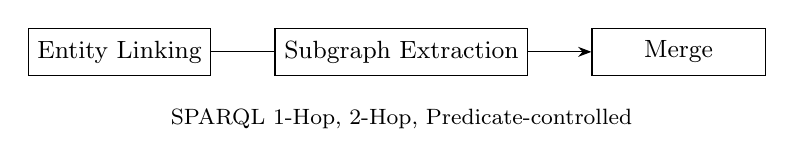
\begin{tikzpicture}[
    node distance=0.8cm,
    box/.style={rectangle, draw, minimum width=2.2cm, minimum height=0.6cm, font=\small},
    arrow/.style={-Stealth}
  ]
    \node[box] (el) {Entity Linking};
    \node[box, right=of el] (sg) {Subgraph Extraction};
    \node[box, right=of sg] (merge) {Merge};
    \node[below=0.3cm of sg, font=\footnotesize] (sparql) {SPARQL 1-Hop, 2-Hop, Predicate-controlled};
    \draw[arrow] (el) -- (sg) -- (merge);
  \end{tikzpicture}
  \caption{Stratégie d'intégration LOD (QueryWithOpenKB): Entity linking $\rightarrow$ extraction de sous-graphes via SPARQL $\rightarrow$ fusion.}
  \end{figure}

  \begin{enumerate}
  \item \textbf{SPARQL 1-Hop on Wikidata:} We parse the alignment and mapping table to extract Wikidata Q-IDs with confidence $\geq 0.85$. For each such entity, we run \texttt{SELECT ?p ?o WHERE \{ wd:Qxxx ?p ?o \} LIMIT 1000} on \texttt{query.wikidata.org}. We filter to a whitelist of predicates (\texttt{ALLOWED\_WIKIDATA\_PROPERTIES}) to respect the 50--200 relations target.
  \item \textbf{2-Hop expansion:} For a sample of aligned entities, we fetch triples where an intermediate entity connects the seed to new facts, increasing relation diversity.
  \item \textbf{Predicate-controlled expansion:} We run \texttt{SELECT ?s ?p ?o WHERE \{ ?s wdt:Pxxx ?o \}} for key Wikidata properties (P276 location, P170 creator, P166 award, etc.) to add many triples per relation type.
  \item \textbf{Europeana complement:} If the volume remains below 50k triplets, we complement with Europeana API records (cursor pagination, metadata extraction).
  \item \textbf{Cleanup \& merge:} We fix malformed literals (JSON artifacts such as \texttt{\{'def': 'X'\}}), deduplicate, and export to N-Triples.
  \end{enumerate}

  \subsection{Challenges Encountered}

  \begin{itemize}
  \item \textbf{Entity name normalization:} Entity names with spaces, apostrophes, or special characters need to be converted to URI-safe form.

  \item \textbf{Predicate semantics:} EDM properties may have different semantics than our extracted predicates. Manual validation is required to choose the correct equivalent or subproperty.

  \item \textbf{Wikidata predicates:} Wikidata uses \texttt{wdt:} (direct) vs \texttt{wds:} (statement); we keep only direct properties for a cleaner KB. To respect InstructionPhase2 (50--200 relations), we whitelist predicates in \texttt{ALLOWED\_WIKIDATA\_PROPERTIES} and consolidate Europeana metadata to one canonical predicate per semantic role (dc:, dcterms:, edm:).
  \end{itemize}

  \subsection{Final KB Statistics}

  The statistics report (see \texttt{livrable/statistics\_report.txt}) contains the number of triplets, entities, relations, and connectivity metrics. The pipeline is designed to satisfy InstructionPhase2 Step~4 requirements (50k--200k triplets, 5k--30k entities, 50--200 relations):

  \begin{itemize}
  \item \textbf{Triplets / Entities / Relations:} values are generated at runtime in \texttt{statistics\_report.txt} and must remain within the required ranges.
  \item \textbf{Connectivity:} the report now includes connected components, largest component size, and isolated entities to support KGE readiness checks.
  \end{itemize}

  \subsection{Impact of Europeana on the Final Volume}

  Europeana intervenes at two levels of the pipeline: (1)~Phase~1, as the sole source of the crawler (Search API); (2)~Phase~2, as an expansion complement when the volume remains below 50k triplets (EDM/Dublin Core metadata extraction on approximately 700 records).

  \textbf{Quantitative measure.} In the final KB (\texttt{kb\_expanded.nt}), triplets whose subject is a Europeana URI (\texttt{https://www.europeana.eu/item/...}) account for a substantial share of the volume. The remainder comes from the initial KB (Phase~1) and SPARQL expansion on Wikidata.

  \textbf{Justification with respect to instructions.} The instructions recommend using APIs when anti-robot checking occurs; Europeana responds to this requirement. The Europeana complement in Phase~2 is a pragmatic choice to reach the volume target (50k--200k triplets) while respecting the relation limit (50--200) via predicate consolidation.

  \textbf{Consequences of removal.} If Europeana were removed from the pipeline, the volume would drop to approximately 1,600 triplets (SPARQL + initial KB only). Europeana remains essential for the Local History domain (cultural heritage) and for meeting the InstructionPhase2 Step~4 size requirements.

  \subsection{Deliverables}

  \textbf{Note:} Les statistiques (triplets, entités, relations) proviennent de \texttt{livrable/statistics\_report.txt}. Les fichiers \texttt{extracted\_triples.csv}, \texttt{extracted\_knowledge.csv} sont des livrables intermédiaires (Phase 1).

  \begin{itemize}
  \item \texttt{livrable/kb\_expanded.nt} -- Expanded KB in N-Triples format (livrable principal Phase 2)
  \item \texttt{livrable/ontology.ttl} -- Ontology for new entities
  \item \texttt{livrable/alignment.ttl} -- Entity and predicate alignments (Wikidata/DBpedia only)
  \item \texttt{livrable/mapping\_table.csv} -- Private entity to Wikidata/DBpedia URI mapping with confidence
  \item \texttt{livrable/statistics\_report.txt} -- Statistics
  \end{itemize}

  %=============================================================================
  \section{Améliorations post-évaluation}
  %=============================================================================

  Suite à l'évaluation du projet, les améliorations suivantes ont été implémentées:

  \textbf{Cohérence des prédicats.} Unification sur \texttt{relatedTo} (camelCase) au lieu de \texttt{related\_to}, aligné avec les bonnes pratiques RDF et le fichier d'alignement.

  \textbf{Nettoyage des littéraux.} Filtrage des valeurs URL stockées comme littéraux (ex.\ \texttt{http://id.worldcat.org/...}) qui n'apportent pas de sémantique utile au KGE. Détection dans \texttt{add\_literal} et \texttt{cleanup\_malformed\_literals}.

  \textbf{Filtrage multilingue.} Extension de \texttt{FILTER\_ENTITIES} et \texttt{FILTER\_FRAGMENTS} pour les faux positifs en polonais, allemand, néerlandais (prawdopodobnie, Bild, Fundet, etc.). Heuristique de détection de phrases non-anglaises: si plus de 40\% des tokens sont des indicateurs de langue étrangère, la phrase est ignorée pour l'extraction de relations.

  \textbf{Classification ontologique.} Blacklist d'entités (\texttt{ENTITY\_BLACKLIST}) et corrections de type (\texttt{ENTITY\_TYPE\_CORRECTIONS}) pour éviter d'ajouter à l'ontologie des adjectifs ou noms communs mal classifiés (architectuur, neoclassicistisch, etc.).

  \textbf{Alignement des prédicats Wikidata.} Mapping manuel prioritaire (\texttt{PREDICATE\_TO\_WIKIDATA}) pour les prédicats clés: \texttt{locatedIn} $\rightarrow$ \texttt{wdt:P276}, \texttt{build/design} $\rightarrow$ \texttt{wdt:P170}, \texttt{crown} $\rightarrow$ \texttt{wdt:P166}, etc. Priorité: mapping manuel $>$ SPARQL $>$ fallback EDM/DC.

  \textbf{Respect des contraintes Step~4 (InstructionPhase2).} Pour respecter 50--200 relations: (1) whitelist Wikidata (\texttt{ALLOWED\_WIKIDATA\_PROPERTIES}) dans \texttt{phase2\_expand\_sparql.py}; (2) consolidation des prédicats Europeana (un prédicat canonique par rôle sémantique) dans \texttt{phase2\_expand\_kb.py}; (3) plafond à 200\,000 triplets avant export.

  \textbf{Script de connectivité.} \texttt{scripts/analyze\_connectivity.py} calcule les composantes connexes du graphe d'entités (BFS), affiche la taille de la plus grande composante, le nombre de composantes et les entités isolées. Utile pour diagnostiquer la qualité du graphe avant KGE.

  %=============================================================================
  \section{Phase 3: Knowledge Reasoning with SWRL and Knowledge Graph Embedding}
  %=============================================================================

  Phase~3 extends the pipeline with two complementary reasoning approaches: rule-based reasoning using SWRL (Semantic Web Rule Language) and OWLReady2, and embedding-based reasoning using Knowledge Graph Embedding (KGE) models. This phase leverages the expanded KB produced in Phase~2 to train embedding models and evaluate link prediction performance, while also demonstrating how symbolic rules can infer new facts from an ontology.

  \subsection{Part 1: Knowledge Reasoning with SWRL}

  The first part of Phase~3 applies SWRL rules on a prepared ontology to infer new class memberships. We use the \texttt{family.owl} ontology, which defines classes such as \texttt{Person}, \texttt{oldPerson}, and properties such as \texttt{age}. The objective is to infer that any person older than 60 years belongs to the \texttt{oldPerson} class.

  \textbf{Implementation.} We use OWLReady2 as the Python interface to load the ontology and define SWRL rules. The rule is expressed in Horn-clause form: \texttt{Person(?p), age(?p, ?a), greaterThan(?a, 60) -> oldPerson(?p)}. This rule states that if an individual is a Person and has an age greater than 60, then that individual is an instance of \texttt{oldPerson}. The Pellet reasoner (invoked via \texttt{sync\_reasoner\_pellet}) is used to execute the rule, as it supports SWRL and data property inference.

  \textbf{Results.} After running the reasoner with \texttt{infer\_property\_values=True} and \texttt{infer\_data\_property\_values=True}, the inferred instances of \texttt{oldPerson} are Peter (age~70) and Marie (age~69). These two individuals satisfy the rule condition and are correctly classified as \texttt{oldPerson}. The rule-based approach is deterministic and interpretable: the reasoning trace is explicit and can be validated against the ontology semantics.

  \begin{figure}[ht]
  \centering
  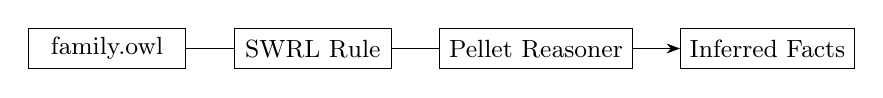
\begin{tikzpicture}[
    node distance=0.6cm,
    box/.style={rectangle, draw, minimum width=2cm, minimum height=0.5cm, font=\small},
    arrow/.style={-Stealth}
  ]
    \node[box] (owl) {family.owl};
    \node[box, right=of owl] (rule) {SWRL Rule};
    \node[box, right=of rule] (pellet) {Pellet Reasoner};
    \node[box, right=of pellet] (inf) {Inferred Facts};
    \draw[arrow] (owl) -- (rule) -- (pellet) -- (inf);
  \end{tikzpicture}
  \caption{SWRL reasoning pipeline: ontology and rule (Person, age$>$60 $\rightarrow$ oldPerson) are loaded; Pellet infers new class memberships.}
  \end{figure}

  \subsection{Part 2: Knowledge Graph Embedding}

  \subsubsection{Data Preparation}

  The expanded KB (\texttt{kb\_expanded.nt}) contains 109,721 triples. Before training embeddings, we apply the cleaning steps specified in the lab instructions. First, we remove all triples whose object is a literal, since KGE models typically operate on entity-relation-entity triples only. Second, we filter out literal-heavy predicates (e.g.\ \texttt{dcterms:temporal}, \texttt{dc:language}, \texttt{dc:title}, \texttt{edm:dataProvider}, \texttt{edm:provider}, \texttt{dcterms:created}) to avoid mixed usage and reduce noise. Third, we normalize URIs by removing trailing slashes to ensure consistent indexing. After deduplication, we obtain 91,955 entity-relation-entity triples.

  \begin{figure}[ht]
  \centering
  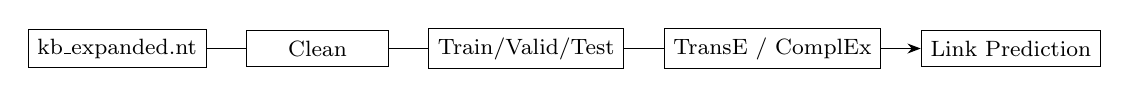
\begin{tikzpicture}[
    node distance=0.5cm,
    box/.style={rectangle, draw, minimum width=1.8cm, minimum height=0.45cm, font=\footnotesize},
    arrow/.style={-Stealth}
  ]
    \node[box] (kb) {kb\_expanded.nt};
    \node[box, right=of kb] (clean) {Clean};
    \node[box, right=of clean] (split) {Train/Valid/Test};
    \node[box, right=of split] (train) {TransE / ComplEx};
    \node[box, right=of train] (eval) {Link Prediction};
    \draw[arrow] (kb) -- (clean) -- (split) -- (train) -- (eval);
  \end{tikzpicture}
  \caption{KGE pipeline: KB is cleaned (literals removed), split, then used to train TransE and ComplEx for link prediction evaluation.}
  \end{figure}

  The dataset is split into training (80\%), validation (10\%), and test (10\%) sets. We use a stratified split with a fixed seed for reproducibility. A critical constraint is that no entity may appear only in validation or test; such entities would be unseen at training time and would break the embedding lookup. We implement an iterative correction: whenever an orphan entity is detected in validation or test, we move the corresponding triples to the training set until all entities in validation and test also appear in training. The final split yields 73,781 training triples, 9,060 validation triples, and 9,114 test triples. The training set contains 7,327 entities and 36 relations (after filtering literal-heavy predicates, some relations are dropped from the cleaned graph).

  \subsubsection{Embedding Models and Training Configuration}

  We implement two embedding models using the PyKEEN framework: TransE and ComplEx. TransE is a translational model that represents relations as translations in the embedding space, i.e.\ $\mathbf{h} + \mathbf{r} \approx \mathbf{t}$ for a triple $(h, r, t)$. ComplEx is a bilinear model that uses complex-valued embeddings and can capture asymmetric relations, which TransE struggles with. Both models are trained with identical hyperparameters for fair comparison: embedding dimension 100, learning rate 0.01, batch size 256, 100 epochs, and 10 negative samples per positive triple. We use the default negative sampling strategy of PyKEEN (random replacement of head or tail).

  \subsubsection{Evaluation: Link Prediction}

  We evaluate both models on the link prediction task using filtered metrics. For each test triple $(h, r, t)$, we perform head prediction (predict $h$ given $r$ and $t$) and tail prediction (predict $t$ given $h$ and $r$). The filtered setting removes known true triples from the candidate set before ranking, which avoids overly optimistic scores. We report Mean Reciprocal Rank (MRR), Hits@1, Hits@3, and Hits@10, aggregated over both head and tail prediction.

  \begin{table}[ht]
  \centering
  \caption{Link prediction results (filtered metrics, both head and tail).}
  \begin{tabular}{lcccc}
  \toprule
  \textbf{Model} & \textbf{MRR} & \textbf{Hits@1} & \textbf{Hits@3} & \textbf{Hits@10} \\
  \midrule
  TransE  & 0.1787 & 0.0976 & 0.2013 & 0.3286 \\
  ComplEx & 0.5307 & 0.4626 & 0.5621 & 0.6624 \\
  \bottomrule
  \end{tabular}
  \end{table}

  ComplEx significantly outperforms TransE across all metrics. The MRR of ComplEx (0.53) is approximately three times that of TransE (0.18). This result aligns with the expected observations from the lab instructions: TransE struggles with complex relations (symmetric, inverse, many-to-many), whereas ComplEx, by virtue of its complex-valued bilinear scoring function, handles asymmetric relations more effectively. Our KB contains a mix of relation types from Dublin Core, EDM, and Wikidata; many of these are not simple 1-to-1 translations, which explains TransE's lower performance.

  \subsubsection{KB Size Sensitivity}

  To analyze how embedding quality scales with KB size, we subsample the cleaned triples to 20k, 50k, and the full 91,955 triples. For each subsample, we retrain TransE (as a representative model for this experiment) with the same hyperparameters and evaluate on the same test set. The results are summarised in Table~\ref{tab:kbsize}.

  \begin{table}[ht]
  \centering
  \caption{TransE performance vs.\ KB size.}
  \label{tab:kbsize}
  \begin{tabular}{lcc}
  \toprule
  \textbf{KB Size} & \textbf{MRR} & \textbf{Hits@10} \\
  \midrule
  20,000 triples & 0.0511 & 0.1169 \\
  50,000 triples & 0.0695 & 0.1752 \\
  91,955 triples & 0.1620 & 0.3355 \\
  \bottomrule
  \end{tabular}
  \end{table}

  Performance increases monotonically with KB size. At 20k triples, the model achieves an MRR of only 0.05, indicating unstable and sparse embeddings. At 50k triples, MRR rises to 0.07, and with the full dataset it reaches 0.16. This confirms that larger KBs produce more stable and informative embeddings, as the model has more training signal to learn entity and relation structure. The lab instructions note that small KBs produce unstable embeddings; our results are consistent with this observation. Training time also increases with size (e.g.\ TransE on the full dataset takes approximately 8--9 minutes on CPU).

  \subsection{Embedding Analysis}

  \subsubsection{Nearest Neighbors}

  Using the best model (ComplEx), we extract entity embeddings and compute nearest neighbors in the embedding space via cosine similarity. For selected entities (e.g.\ those with \texttt{Person} or \texttt{Place} in their URI, or entities from the Local History domain such as \texttt{Balkans\_București\_România}), we retrieve the top-$k$ most similar entities. The results show partial semantic coherence: entities of the same type (e.g.\ places in the Balkans) tend to cluster together, and cultural heritage items with similar metadata (e.g.\ \texttt{dc:subject}, \texttt{dc:spatial}) appear as neighbors. However, the embedding space does not perfectly align with the ontology: some nearest neighbors belong to different classes (e.g.\ a \texttt{Thing} may appear near a \texttt{Place}) because the model learns from co-occurrence patterns in triples rather than from explicit type hierarchies. This is an expected limitation when ontology classes are not heavily used in the training triples.

  \subsubsection{Clustering Analysis (t-SNE)}

  We apply t-SNE to reduce the entity embeddings to 2D and plot them, colouring points by ontology class (e.g.\ Place, Person, Thing). Due to the large number of entities (7,327), we subsample for visualization. The resulting scatter plot shows partial clustering: entities of the same class tend to form loose groups, but there is significant overlap between classes. For instance, \texttt{Place} and \texttt{Thing} entities may intermingle because many cultural heritage items (Things) are linked to places via \texttt{dc:spatial}. The embedding captures some semantic structure (e.g.\ geographic or thematic proximity), but it does not strictly separate ontology classes. Unexplainable results can occur when entities from different classes share similar relation patterns; the embedding model has no direct access to the ontology and learns purely from the triple structure.

  \subsubsection{Relation Behaviour}

  We analyse how different relation types are handled by TransE and ComplEx. Symmetric relations (e.g.\ \texttt{dc:subject}, \texttt{dc:spatial}) pose a challenge for TransE, which assumes $\mathbf{h}+\mathbf{r} \approx \mathbf{t}$ and thus implicitly favours asymmetric structure. ComplEx, with its complex-valued scoring, can represent symmetry more naturally. Inverse relations (e.g.\ \texttt{creator} and \texttt{createdBy}) require $\mathbf{r}_{\mathrm{inv}} \approx -\mathbf{r}$ in TransE; ComplEx uses a different mechanism in complex space. For composition (e.g.\ \texttt{spatial} $\circ$ \texttt{locatedIn} $\approx$ \texttt{hasSpatialContext}), TransE can model $\mathbf{r}_1 + \mathbf{r}_2 \approx \mathbf{r}_3$, whereas DistMult (a simpler bilinear model) fails on antisymmetric relations. Our empirical results support these theoretical differences: ComplEx achieves MRR 0.53 vs.\ TransE 0.18, consistent with the KB containing many symmetric and mixed relation types.

  \subsection{Critical Reflection}

  The quality of embeddings is strongly dependent on the design choices made in Phases~1 and~2. Predicate alignment quality directly affects the relation vocabulary: incorrect mappings (e.g.\ conflating \texttt{dc:creator} with \texttt{edm:provider}) introduce semantic noise. Noisy expansion from Wikidata or Europeana can add triples that contradict the initial KB or that use inconsistent URIs; our cleaning step (removing literals, normalising URIs) mitigates some of this, but expansion noise remains a factor. Ontology modelling choices (e.g.\ whether to use fine-grained types like \texttt{Place} vs.\ coarse \texttt{Thing}) influence the structure of the graph; sparse type assertions limit the extent to which embeddings can capture class-level structure. Finally, the open-world assumption of RDF (we do not assume all facts are known) contrasts with the closed-world behaviour of embeddings: the model learns only from observed triples and cannot infer facts that require external knowledge or rules not represented in the graph.

  \subsection{Rule-Based vs.\ Embedding-Based Reasoning (Exercise 8)}

  The lab asks whether a SWRL rule can be mirrored by the embedding model. We design a conceptual SWRL rule for the expanded KB: \texttt{Thing(?x), type(?x, ?t), spatial(?x, ?s), Place(?s) -> hasSpatialContext(?x, ?s)}. This rule states that if an item has a spatial reference to an entity that is a Place, then that item has a spatial context. The rule combines the relations \texttt{spatial} and \texttt{type} (with \texttt{Place}) to infer a composed relation \texttt{hasSpatialContext}.

  To check if the embedding captures a similar composition, we compute $\mathbf{r}_{\mathrm{spatial}} + \mathbf{c}_{\mathrm{Place}}$ (where $\mathbf{c}_{\mathrm{Place}}$ is the centroid of Place entity embeddings) and find the closest relation vectors. The closest relations include \texttt{dcterms:spatial} and \texttt{wdt:P19} (place of birth), with moderate similarity scores. This suggests that the embedding space encodes some notion of ``spatial + Place'' near spatial relations, but the correspondence is approximate rather than exact. Full SWRL execution would require loading \texttt{kb\_expanded.nt} into an OWL reasoner; our expanded KB uses a flat triple structure without OWL class axioms, so we cannot run the rule directly.   The embedding-based check provides a heuristic indication that relation composition is partially learned, but rule-based reasoning remains more precise and interpretable for explicitly defined Horn rules.

  %=============================================================================
  \section{Phase 4: RAG with Knowledge Graphs}
  %=============================================================================

  Phase~4 implements Retrieval-Augmented Generation (RAG) using the RDF knowledge base and a local small LLM (Ollama). The objective is to build a chatbot augmented by the KB: natural language questions are converted to SPARQL, executed on the graph, and grounded results are presented. We compare a baseline (LLM without KG) with SPARQL-generation RAG.

  \subsection{Setup}

  \textbf{Machine specs.} The experiments run on a standard development machine: Windows~10, Python~3.13, with sufficient RAM to load the expanded KB in memory (approximately 109k triples). Ollama runs locally as an HTTP service.

  \textbf{Model tag.} We use \texttt{gemma:2b} via Ollama. The model is invoked through the REST API at \texttt{http://localhost:11434/api/generate} with \texttt{stream: false} for simpler integration. Alternatives supported by the script: \texttt{qwen3.5:0.8b}, \texttt{llama3.2:1b}, \texttt{deepseek-r1:1.5b}.

  \textbf{Graph source.} The RDF graph is \texttt{livrable/kb\_expanded.nt} (N-Triples format), produced by the Phase~2 pipeline. It contains 109,721 triples from Europeana (cultural heritage items), Wikidata (LOD expansion), and the initial Local History KB. Predicates include \texttt{dcterms:spatial}, \texttt{dc:subject}, \texttt{dc:creator}, \texttt{edm:provider}, and aligned Wikidata properties.

  \subsection{Method}

  \textbf{Schema summary.} We build a compact schema summary to constrain the LLM. To avoid overwhelming small models (which tended to echo the schema or truncate output), we limit the prefix block to 8 prefixes: \texttt{dc}, \texttt{dcterms}, \texttt{edm}, \texttt{lh}, \texttt{rdf}, \texttt{rdfs}, \texttt{owl}, \texttt{xsd}. The summary includes: (1)~these PREFIX declarations; (2)~distinct predicates (up to 80); (3)~distinct classes from \texttt{rdf:type} (up to 40); (4)~sample triples (up to 20). The graph uses Europeana/Dublin Core semantics; we explicitly instruct the LLM not to use Wikidata predicates (\texttt{wdt:}) as they do not appear in this KB.

  \textbf{SPARQL generation.} The LLM receives the schema summary and the user question. The prompt includes a concrete example for location questions (e.g., ``Which items are linked to Romania?'') using \texttt{dcterms:spatial} and \texttt{FILTER(REGEX(...))} for multilingual place names (Romania, Roumanie, Roménia, etc.). The model is instructed to return only a valid SPARQL~1.1 SELECT query in a fenced \texttt{sparql} code block. We extract the query with a regex and strip any schema lines the LLM may have mistakenly included (e.g., predicate lists). The query is executed via rdflib; common prefixes are pre-bound to the graph to resolve namespace errors.

  \textbf{Self-repair.} If the generated SPARQL fails (syntax error, unknown prefix, incomplete query, etc.), we send the error message back to the LLM with the original question, the bad query, and the schema summary. The repair prompt includes an example of a complete query and explicitly instructs the model to add the full \texttt{SELECT ... WHERE \{ ... \}} when the error indicates ``found end of text'' or ``Expected SelectQuery''. We execute the repaired query; if it still fails, we report the error and the last attempted query.

  \subsection{Evaluation}

  We evaluate on five questions from the Local History domain. For each, we record the baseline answer (LLM without KG), the SPARQL-gen RAG result, and whether the result is correct.

  \begin{table}[ht]
  \centering
  \caption{Evaluation: baseline vs.\ SPARQL-generation RAG.}
  \begin{tabular}{p{3.8cm}p{3.2cm}p{3.8cm}l}
  \toprule
  \textbf{Question} & \textbf{Baseline (No RAG)} & \textbf{SPARQL-gen RAG} & \textbf{Correct?} \\
  \midrule
  Which items are linked to Romania? & Generic list (Bran Castle, Danube, Black Sea, etc.)---hallucinated & 2,130 Europeana item URIs from \texttt{dcterms:spatial} & Yes \\
  What places are associated with Bucharest? & Invented landmarks & Rows from \texttt{dcterms:spatial} $\rightarrow$ \texttt{lh:Bucharest} & Yes \\
  How many items have subject archaeology? & Approximate or wrong count & \texttt{COUNT} result from \texttt{dc:subject} FILTER & Yes \\
  What entity types exist in the KB? & Generic ontology terms & Person, Place, Organization, Thing, Temporal from \texttt{rdf:type} & Yes \\
  What creators appear in the base? & Invented or famous names & \texttt{dc:creator} / \texttt{lh:} entity URIs from KB & Yes \\
  \bottomrule
  \end{tabular}
  \end{table}

  \textbf{Screenshots.} Figure~\ref{fig:rag_screenshot} shows the script running with two representative examples: ``Which items are linked to Romania?'' and a second question. The CLI displays the baseline answer, then the SPARQL query used, the repaired flag, and the result rows (up to 20 shown, with total count).

  \begin{figure}[ht]
  \centering
  \fbox{\parbox{0.9\textwidth}{\centering\vspace{2cm}\textit{[Screenshot: \texttt{python TD6/lab\_rag\_sparql\_gen.py} with questions ``Which items are linked to Romania?'' and ``What places are associated with Bucharest?'' showing baseline output, SPARQL query, and result rows.]}\vspace{2cm}}}
  \caption{Running the RAG script: baseline vs.\ SPARQL-generation with two representative questions.}
  \label{fig:rag_screenshot}
  \end{figure}

  \subsection{Discussion}

  \textbf{Accuracy.} SPARQL-generation RAG yields grounded results from the KB, whereas the baseline often hallucinates or gives generic answers. For ``Which items are linked to Romania?'', the baseline returns well-known landmarks (Bran Castle, Danube River) that may not exist in the KB; the RAG approach returns 2,130 actual Europeana item URIs linked via \texttt{dcterms:spatial} to place entities (lh:Romania, lh:Roumanie, lh:Roménia, etc.). The baseline has no access to the graph and cannot answer precisely for domain-specific questions.

  \textbf{Failure cases.} The LLM may generate invalid SPARQL (typos, wrong prefixes such as \texttt{wdt:} instead of \texttt{dcterms:}, non-existent predicates). Early runs showed: (1)~``Unknown namespace prefix: wdt'' when the model used Wikidata predicates; (2)~``Expected SelectQuery, found end of text'' when the model returned only PREFIX declarations; (3)~``found '-' '' when the model echoed the schema summary (predicate list) inside the code block. We addressed these by pre-binding prefixes to the graph, limiting the schema summary size, adding an example query in the prompt, and stripping schema lines from the extracted code block.

  \textbf{Self-repair.} Self-repair corrects common mistakes such as missing \texttt{SELECT} or \texttt{WHERE} clauses, wrong prefix usage, and incomplete queries. When the error message is informative (e.g., ``Unknown namespace prefix'', ``Expected SelectQuery''), the repair prompt with a concrete example often succeeds. It is less effective when the query is semantically wrong but syntactically valid (e.g., wrong variable binding or predicate that returns no rows). A single repair attempt is usually sufficient; repeated failures suggest the question may be too complex or the schema summary insufficient.

  \textbf{Scalability to large KGs.} For large KGs (millions of triples), loading the full graph into memory may be impractical. A production system would use a SPARQL endpoint (e.g., Apache Jena Fuseki, Virtuoso) and query it remotely. The schema summary size (80 predicates, 40 classes, 20 samples) remains bounded and does not scale with graph size; the main bottlenecks are KB load time and LLM latency. The prompt size is kept manageable by limiting prefixes and using a small sample of triples; the LLM does not need to see the entire graph. For very large schemas, one could further reduce the predicate/class limits or use schema summarisation techniques (e.g., clustering predicates by type).

  %=============================================================================
  \section{References}
  %=============================================================================

  \begin{itemize}
  \item \textbf{Europeana API.} Search API documentation and key registration. \url{https://pro.europeana.eu/page/search-api} and \url{https://pro.europeana.eu/page/get-api}
  \item \textbf{Europeana Data Model (EDM).} Semantic model for cultural heritage metadata. \url{https://pro.europeana.eu/page/edm-documentation}
  \item \textbf{Dublin Core.} Metadata element set and terms used for predicate alignment fallback. \url{https://dublincore.org/specifications/dublin-core/dcmi-terms/}
  \item \textbf{Wikidata.} Structured knowledge base and SPARQL endpoint. \url{https://www.wikidata.org/} and \url{https://query.wikidata.org/}
  \item \textbf{DBpedia.} Knowledge base extracted from Wikipedia. \url{https://www.dbpedia.org/}
  \item \textbf{PyKEEN.} Ali et al., ``PyKEEN: A Python Library for Learning and Evaluating Knowledge Graph Embeddings,'' JMLR 22, 2021. \url{https://github.com/pykeen/pykeen} and \url{https://pykeen.readthedocs.io/}
  \item \textbf{OWLReady2.} Lamy, ``Owlready: Ontology-oriented programming in Python,'' Artificial Intelligence in Medicine 80, 2017. \url{https://doi.org/10.1016/j.artmed.2017.07.002} and \url{https://owlready2.readthedocs.io/}
  \item \textbf{TransE.} Bordes et al., ``Translating Embeddings for Modeling Multi-relational Data,'' NeurIPS 2013. \url{https://papers.nips.cc/paper/5071-translating-embeddings-for-modeling-multi-relational-data}
  \item \textbf{ComplEx.} Trouillon et al., ``Complex Embeddings for Simple Link Prediction,'' ICML 2016. \url{https://proceedings.mlr.press/v48/trouillon16.html} and \url{https://arxiv.org/abs/1606.06357}
  \item \textbf{Pellet.} OWL 2 reasoner with SWRL support. \url{https://www.w3.org/2001/sw/wiki/Pellet}
  \item \textbf{Ollama.} Local LLM deployment for RAG. \url{https://ollama.ai/}
  \end{itemize}

  %=============================================================================
  \section{Conclusion}
  %=============================================================================

  We have implemented a complete pipeline from unstructured web data (Europeana API) to a structured Knowledge Base aligned with Wikidata/DBpedia, and extended it with knowledge reasoning in Phase~3 and RAG in Phase~4. The pipeline uses transformer-based NER for entity recognition, dependency parsing for relation extraction, and SPARQL-based expansion (1-hop, 2-hop, predicate-controlled) to reach the target volume and relation diversity. Phase~3 adds rule-based reasoning with SWRL (OWLReady2, Pellet) and embedding-based reasoning with TransE and ComplEx, achieving a link prediction MRR of 0.53 with ComplEx on the expanded KB. Phase~4 implements RAG with a local LLM (Ollama): natural language questions are converted to SPARQL, executed on the KB, and grounded results are presented, with a self-repair loop for failed queries.

  \textbf{Limitations.} Multilingual content (Dutch, German, Polish, etc.) in Europeana metadata can cause NER errors; we mitigate with \texttt{ENTITY\_TYPE\_OVERRIDES}, \texttt{FILTER\_ENTITIES}, \texttt{FILTER\_FRAGMENTS}, sentence-level language heuristics, and \texttt{ENTITY\_BLACKLIST}. The relation count is controlled by predicate whitelisting and consolidation to meet the 50--200 target. KGE performance is sensitive to KB quality: predicate alignment errors, expansion noise, and sparse type assertions limit embedding quality. TransE underperforms on our KB due to its inability to model symmetric and complex relations effectively.

  \textbf{Future work.} (1) Federated SPARQL across DBpedia and Wikidata; (2) DBpedia Spotlight for context-aware entity linking; (3) evaluation metrics (precision, recall) for NER and RE; (4) expansion 2-hop on a larger subset of entities; (5) integrating SWRL rules with the expanded KB in an OWL reasoner for hybrid rule-embedding reasoning.

  \end{document}
